\documentclass[tikz,border=4pt]{standalone}
\usepackage[T1]{fontenc}
\usepackage{mathptmx}
\usetikzlibrary{arrows.meta,calc,decorations.pathreplacing,decorations.pathmorphing}
\begin{document}
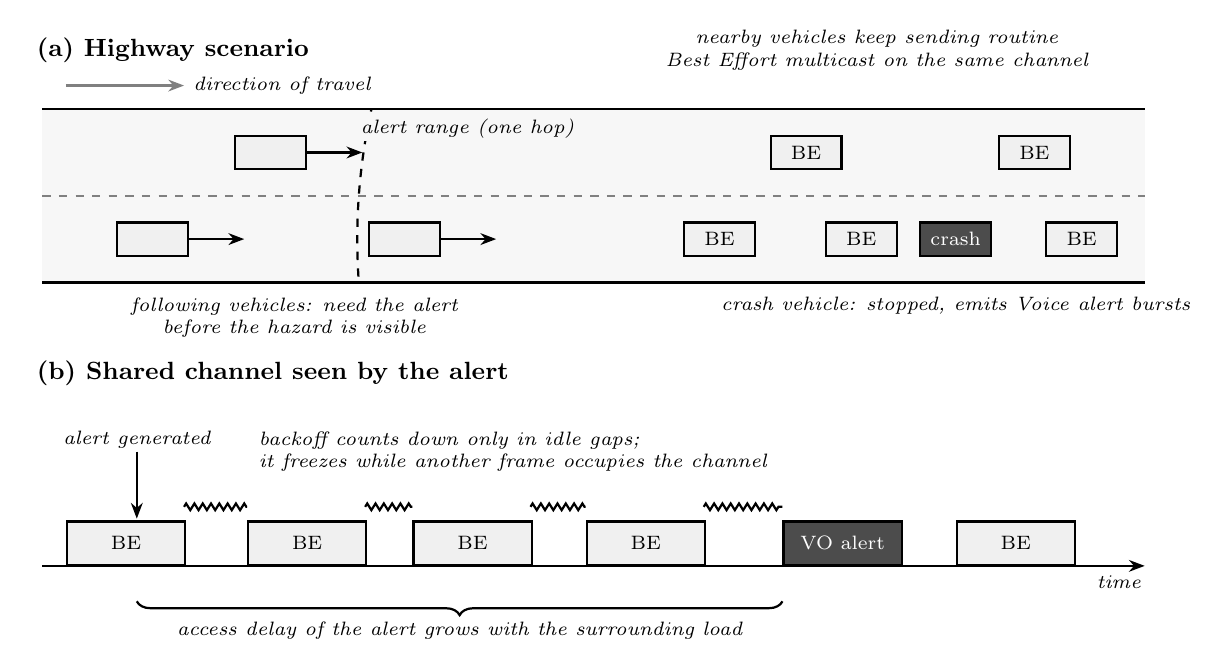
\begin{tikzpicture}[
  font=\footnotesize,
  >=Stealth,
  thick,
  car/.style={draw, thick, fill=black!6, minimum width=0.9cm, minimum height=0.42cm, inner sep=0pt, font=\scriptsize},
  crash/.style={car, fill=black!70, text=white},
  frame/.style={draw, thick, minimum height=0.55cm, inner sep=0pt, font=\scriptsize},
  be/.style={frame, fill=black!6},
  vo/.style={frame, fill=black!70, text=white},
  arr/.style={-{Stealth[length=2.0mm]}, thick},
  lab/.style={font=\scriptsize\itshape, align=center, inner sep=1pt},
  ptitle/.style={font=\small\bfseries, anchor=west},
]

  % ===== (a) Road scenario =====
  \node[ptitle] at (-0.2,4.55) {(a) Highway scenario};
  \fill[black!3] (0,1.6) rectangle (14,3.8);
  \draw[thick] (0,1.6) -- (14,1.6);
  \draw[thick] (0,3.8) -- (14,3.8);
  \draw[thick, dashed, black!50] (0,2.7) -- (14,2.7);
  \draw[arr, black!50] (0.3,4.1) -- (1.8,4.1) node[lab, right=2pt, black] {direction of travel};

  % alert range of the crash vehicle
  \begin{scope}
    \clip (0,1.6) rectangle (14,3.8);
    \draw[thick, dashed] (11.6,2.15) circle (7.6cm);
  \end{scope}
  \node[lab, fill=black!3] at (5.4,3.55) {alert range (one hop)};

  % crash vehicle
  \node[crash] (cv) at (11.6,2.15) {crash};
  \node[lab] at (11.6,1.3) {crash vehicle: stopped, emits Voice alert bursts};

  % neighbours near the crash, transmitting Best Effort
  \foreach \x/\y/\n in {9.7/3.25/n1, 10.4/2.15/n2, 12.6/3.25/n3, 8.6/2.15/n4, 13.2/2.15/n5}{
    \node[car] (\n) at (\x,\y) {BE};
  }

  % following vehicles approaching
  \node[car] (f1) at (4.6,2.15) {};
  \node[car] (f2) at (2.9,3.25) {};
  \node[car] (f3) at (1.4,2.15) {};
  \draw[arr] (f1.east) -- ++(0.7,0);
  \draw[arr] (f2.east) -- ++(0.7,0);
  \draw[arr] (f3.east) -- ++(0.7,0);
  \node[lab, align=center] at (3.2,1.15) {following vehicles: need the alert\\before the hazard is visible};
  \node[lab, align=center] at (10.6,4.55) {nearby vehicles keep sending routine\\Best Effort multicast on the same channel};

  % ===== (b) Channel timeline =====
  \node[ptitle] at (-0.2,0.45) {(b) Shared channel seen by the alert};
  \def\yb{-1.6}
  \draw[arr] (0,\yb-0.4) -- (14,\yb-0.4) node[lab, anchor=north east, yshift=-2pt] {time};

  \node[be, minimum width=1.5cm, anchor=south west] at (0.3,\yb-0.4) {BE};
  \node[be, minimum width=1.5cm, anchor=south west] at (2.6,\yb-0.4) {BE};
  \node[be, minimum width=1.5cm, anchor=south west] at (4.7,\yb-0.4) {BE};
  \node[be, minimum width=1.5cm, anchor=south west] at (6.9,\yb-0.4) {BE};
  \node[vo, minimum width=1.5cm, anchor=south west] (voF) at (9.4,\yb-0.4) {VO alert};
  \node[be, minimum width=1.5cm, anchor=south west] at (11.6,\yb-0.4) {BE};

  % alert generated
  \draw[arr] (1.2,\yb+1.05) -- (1.2,\yb+0.2);
  \node[lab, above=0pt] at (1.2,\yb+1.05) {alert generated};

  % backoff countdown in idle gaps, frozen during busy periods
  \foreach \a/\b in {1.8/2.6, 4.1/4.7, 6.2/6.9, 8.4/9.4}{
    \draw[thick, decorate, decoration={zigzag, amplitude=1.2pt, segment length=3pt}] (\a,\yb+0.35) -- (\b,\yb+0.35);
  }
  \node[lab, align=left, anchor=west] at (2.7,\yb+1.05) {backoff counts down only in idle gaps;\\it freezes while another frame occupies the channel};

  \draw[decorate, decoration={brace, mirror, amplitude=5pt}, thick] (1.2,\yb-0.85) -- (9.4,\yb-0.85)
    node[lab, midway, below=6pt] {access delay of the alert grows with the surrounding load};
\end{tikzpicture}
\end{document}
